% !TEX root =  main.tex
\newcommand{\sys}{ProcIterRoles}

\section{ProcIteRoles Architecture}
\begin{figure}[hbt]
	\begin{center}
	%6.44 x 3.99
	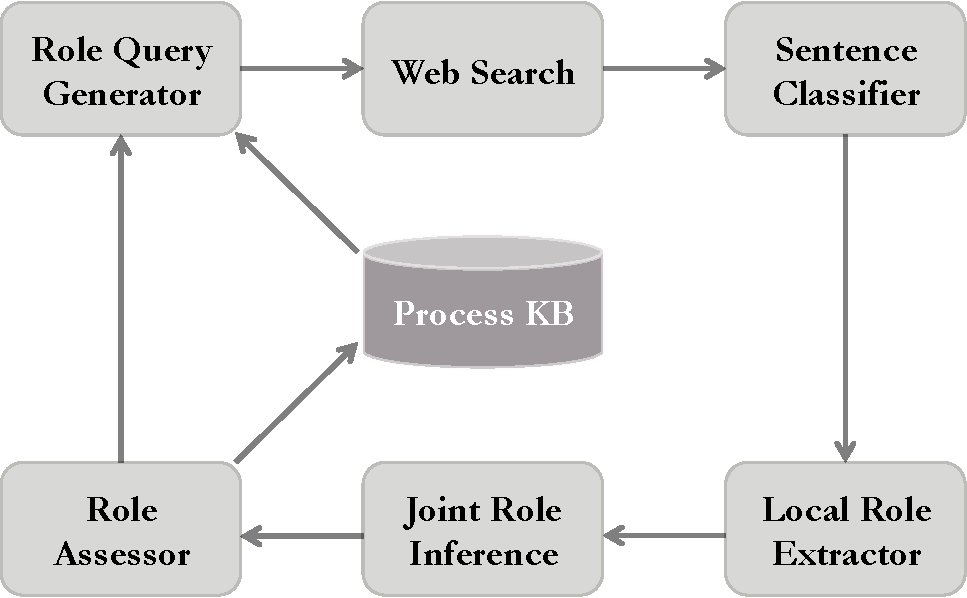
\includegraphics[width=3.22in,height=1.99in]{figures/architecture.pdf} 	
	\caption{\label{fig:architecture} {Process KB Acquisition: Proposed Architecture}}
	\end{center}
\end{figure}
\sys\ allows for targeted iterative acquisition and refinement of process roles.
The main idea is to collect high quality sentences and roles and iteratively expand the acquisition to include
additional sentences and other roles. 

Figure~\ref{fig:architecture} shows the architecture of the acquisition process. 
Using simple query patterns we search for sentences that express roles with highly regular lexical cues. 
A sentence filter addresses sense issues and to remove malformed sentences.
The filtered sentences are then processed through a pattern-based extractor that identifies and scores the candidate roles. 
In parallel, the sentences are also aligned to identify lexical units that should play similar semantic roles in the sentences. 
A joint inference module then provides a collective label assignment for all the sentences. 
The extracted roles are then assessed in conjunction with the existing roles. 
The assessor determines which roles should be added to the KB and also determines which roles need further additions. 
New query patterns are created for the roles that need addition and whole procedure is repeated again. 

In the subsequent sections, we describe each component in greater detail.

\section{Sentence Gathering}

\sys\ will leverage the vastness of the web to build a targeted collection of sentences that expresses roles of interest.
There are two key challenges to address in gathering relevant sentences:
\begin{itemize}
\item {\bf Relevance} -- We want to find sentences that describe the target process of interest. 
The vastness of the web also means that there is information on nearly any possible interpretation of the words used to describe the process. 
For instance if we are interested in the process {\em crop fertilization}, we might also find information on {\em fertilization} in the reproductive sense, 
or in other metaphorical uses such as {\em cross fertilization of ideas}. 
Also, the target sense may not be a dominant sense on the web. 
Constructing effective keyword queries is therefore critical for finding relevant information.
\item {\bf Role Coverage} -- We want to find sentences that cover all applicable roles that convey the desired information via simple expected constructions.
Some roles are often expressed via highly regular lexico-syntactic constructions. 
On the other hand, roles such as {\em x} can be expressed in many different ways. 
Again with the vastness of the web, constructing effective role patterns is critical for finding useful sentences. 
\end{itemize}

To address these challenges we propose two strategies. First, we target definitional sentences which convey the most salient information. Second, we espouse a feedback strategy that leverages high quality sentences gathered in the earlier phases to guide search in the later stages.

\subsection{Querying}

We propose to investigate simple but effective query pattern formulation methods. 
On a related task, our prior work had explored techniques that can find sentences that convey information about different aspects with respect to a topic (e.g., biographical aspects of a person). 
Our preliminary work shows that simple lexical templates e.g., "<process name> is the process by which" can yield high quality {\em definitional} sentences about processes. 
We use additional lexical templates for roles with regular lexicon-syntactic constructions e.g., "<process name> causes" is an effective pattern to find sentences that express the {\em result} roles of processes. The key challenge is to figure out querying patterns for roles with diverse lexical realizations. We propose adopting the standard bootstrapping approach used in relation extraction techniques to borrow functional patterns that introduce roles in other processes. Bootstrapping is known to introduce noise and topic drift issues. However, our approach doesn't entirely rely on the patterns alone. Rather we propose strong scoring and filtering mechanisms that can remove noise introduced via bootstrapping.

\subsection{Scoring and Filtering}

To account for the challenges in relevance, we seek to build a distributional context model that is seeded with some domain corpus. This model is then refined iteratively to allow for role coverage. 
Sentences from the web have high variance in quality and relevance. 

\section{Role Extraction}

Many different approaches have been investigated for role labeling.
The learning formulations studied range from pipelined classification approaches~\cite{gildea2002automatic,bjorkelund2009multilingual}, 
efficient structured and joint inference~\cite{koomen2005generalized,tackstrom2015efficient}, to end-to-end deep learning architectures~\cite{foland2015dependency}.
Many different lexico-syntactic features, such as dependency paths and n-gram contexts, provide weak evidences for determining semantic roles~\cite{gildea2002automatic}. 
Because these path-based and n-gram features are sparse, these supervised techniques require large amounts of training data. 
Semi-supervised and unsupervised approaches have been proposed as a means to address the training data problem~\cite{furstenau-emnlp2009,klementievsemi}.

The focus of these approaches have been to build a SRL system that can identify the roles mentioned in a sentence. 
Our requirement is subtly different. We need to build a mechanism for acquiring the typical role fillers for a given process. 
First, we formulate a simpler local classification task that avoids the need for learning over role and predicate specific patterns. 
Starting with sentences that are likely to contain a specific role and a candidate text span from the sentence, 
we pose a classification task to determine if the candidate  is indeed expressing role of interest. 
Then, we pose a joint inference task over multiple sentences, which allows us to use role decisions on similar 
text spans to influence each other. 

\subsection{Local Role Extraction}

We set up a local (within sentence per role) extraction task. Relying on the patterns alone is problematic. Hand authored patterns, especially specifying the expected syntactic structure of the argument is quite limiting. Instead we generate many possible arguments that match a range of weakly indicative argument patterns and train a classifier. 

The inputs are a sentence $S$, the role $R$ for which it was retrieved, and the role pattern $X_R$ that it matches, and a set of candidate spans $C$.
The task is to predict if for each span if it is expressing the role of interest. 

We adopt the standard SRL features such as clause, dependency path features, and n-gram context features~\cite{gildea2002automatic,koomen2005generalized}. 
We explore two types of extensions that are specific to our setting:
\begin{itemize}

\item Different from a standard SRL setting, we seek identification of roles with respect to a canonical realization of the process. 
One can view this task as finding a mapping from predicate-specific semantic role to the process-specific role. 
To this end, we use an SRL system trained on PropBank data to identify predicate level semantic roles and use those as features to derive this mapping.
Similarly, the frames that are evoked by the predicates in the sentence also provide important signals. For example, knowing that there is a conversion 
frame in a sentence increases the possibility of finding a result of a change of state of process like evaporation. 

\item Also we have strong expectations on {\em how} the argument is realized because the sentence is retrieved via a specific query pattern.
This allows us to encode features that test if the expectations are met. [{\bf Explain w/ an example}]

\end{itemize}


%Rather than focus on joint role inference at a sentence level, we explore joint inference across sentences.
%This task is different from the standard SRL setting in two ways. 
%First, we have a strong expectation on {\em how} the argument is realized because the sentence is retrieved via a specific query pattern.
%This allows us to encode features that test if the expectations are met. 
%Second, the task of identifying roles is not specific to a particular predicate. 
%Rather, the roles are identified with respect to a canonical realization of the process. 
%One can view this task as that of mapping from the predicate-specific semantic role to the process-specific role. 

\subsection{Joint Role Inference}

Within sentence joint role inference has been shown to help SRL~\cite{punyakanok2004srl,koomen2005generalized}.
Since our objective is to extract knowledge from multiple sentences, we propose to also exploit joint inference of roles across sentences. Local role extraction allows to reliably identify whether the specified role is expressed by the candidate text spans. However, this local classification is often inadequate because some cue patterns are ambiguous. For example, "evaporates into <x>" can match "steam" which is a {\em result} or "atmosphere" which is a {\em location}. Relying on the extraction pattern alone is problematic. Therefore, we propose to leverage role predictions on other similar text spans to improve inference. 


{\bf Formalism}

The key premise is that aligned text spans in similar sentences should be assigned same roles. This idea had been successfully used in semi-supervised and unsupervised settings to increase training data for SRL~\cite{furstenau-emnlp2009,furstenau2012semi,lang-emnlp2011}. We adopt it for joint inference over test sentences, similar to the transductive learning approaches~\cite{?}.

We extend an ILP-based formalism which has been shown to successfully model within sentence joint inference for SRL~\cite{punyakanok2004srl}. We add 1) a penalty term to the maximization objective that penalizes assignments that violate smoothness of labeling, 2) constraints that effectively fix labels from the local extractor for certain roles. 

As noted earlier, the local extractor scores each text span $t_{i,k}$ from sentence $S_k$ on how likely it is to belong to the role $r_j$. We use indicator variables to denote role assignment. $z_{ijk}$ represents if the text span $t_{ik}$ in sentence $S_k$ is assigned the role $r_j$. Formally, the inference aims to find the best joint assignment to set of indicator variables $\mathbb{z}$ that maximizes the following objective function:

\begin{align*}
%\sum_{t_{ik}} \sum_{r_j} 
 \arg\max_{\mathbf{z}}  \sum_{i,j,k} z_{ijk} \cdot \rho(t_{ik}, r_j) \cdot \lambda_{j}
	&- \beta \left\{ \sum_{i,k,l,m} \sigma(t_{ik}, t_{lm}) \left(\sum_{c \in |R|} |z_{ick} - z_{lcm}| \right) \right\}\\
\mbox{subject to} \\
\forall z_{ick} \in \mathbf{z}, \sum_{c = 1}^{|R|} z_{ick} \le 1  &\mbox{[A span gets only one role.]}\\
\forall S_k \forall c \in |R|, \sum_{t_{ik} \in S_k} z_{ick} \le 1  & \mbox{[Roles are not repeated.]} \\
 \cdots&  \mbox{[Other within sentence constraints.]}
\end{align*}

{\bf Alignment}

The effectiveness of the joint inference relies on the ability to identify text spans in different sentences that should get the same role. 
Prior work explored a dependency graph-based approach to align predicate-argument structures in sentences. A linear combination of the overlap in lexical and syntactic structures of the candidate text spans is used to evaluate whether they should get the same roles~\cite{furstenau-emnlp2009,furstenau2012semi,lang-naacl2010}.
This scoring function is used to transfer roles from a labeled sentence to an unlabeled sentence (semi-supervised setting) or to induce roles as clusters of arguments (unsupervised setting). 

A key difference in our setting is that there are different sub-groups of sentences with different alignment characteristics. 
{\em Definition} sentences describe the process in terms of classes of entities and {\em instance} sentences which involve specific entities.
Aligning definitional sentences is quite different from aligning definitions with instances or instances with other instances. 
Instances involve completely different entities which may not align via direct entailment but may align as substitutable siblings.
Also, instances often tend to involve other non-essential information with respect to the process, 
whereas definitions are compact and tend to contain the most salient bits of information. 
To account for these differences we consider two extensions. Use different sets of weights and different similarity functions to combine the scores based on the types of sentences being aligned.

\begin{align*}
\sigma(t_{ik}, t_{lm}, u, v)	= \alpha_{uv} \cdot lexsim_{uv}(t_{ik}, t_{lm}) + (1 - \alpha_{uv}) \cdot synsim_{uv}(t_{ik}, t_{lm})\\
\end{align*}

[{\bf Consider changing this to a trained classifier. Use sentence patterns rather than definition or instance sentence distinction.}]

\eat{

[{\bf To be redone. Emphasize role discovery.}]
Inference yields a set of roles that can be reliably identified from the input set of sentences. 
The knowledge thus gathered is limited by the query patterns that we used to retrieve the sentences in the first place. 
To expand the knowledge further, we propose an iterative procedure that learns from the inferred roles. 

\subsection{Aggregation}
First, given the current state of the knowledge base and newly inferred roles we devise a simple aggregation procedure that consolidates the roles -- resolving any inconsistencies between the different iterations\footnote{
It is possible to infer new roles with respect to the KB at each iteration, it can introduce many variables 
in inference and render it inefficient.
}.

\subsection{Assessment}

We inspect the KB to identify roles that apply for a specific process based on the confidences of the inferred roles. 
Note that we do not make any assumptions a priori about what roles apply to a process. 
Further not all roles maybe covered by the roles vocabulary. For example, ....
We identify regular syntactic signatures that are not classified into existing roles and use them to derive new knowledge.


need to be filled, and pass them on to the sentence gathering components for expansion.
}

%instantiate new patterns to identify better sentences. The idea is to evaluate lexical alternatives that can form better queries to identify sentences. For example, sentences describing instances of conduction of heat are better found by adding {\em heat}. This type of query expansion using pseudo-relevance feedback is a well studied technique in information retrieval. We consider a restricted version of this problem, where are looking to instantiate existing query templates. 




